\documentclass[border=8pt]{standalone}
\usepackage{xcolor}
\usepackage{pgfplots}
\usepgfplotslibrary{fillbetween, groupplots}
\usetikzlibrary{positioning, calc}
\pgfplotsset{compat=1.18}
\usepackage{amsmath}
\usepackage{graphicx}

\definecolor{algcol0}{HTML}{3B7BC8}
\definecolor{algcol1}{HTML}{7B6EBF}
\definecolor{algcol2}{HTML}{389C56}
\definecolor{algcol3}{HTML}{E63946}

\pgfplotsset{
  size plot/.style={
    width=5.8cm,
    height=5.8cm,
    grid=both,
    xmode=log,
    log basis x={2},
    xmin=1.6245,
    xmax=78.7932,
    grid style={line width=0.35pt, draw=gray!35},
    xtick={2,4,8,16,64},
    xticklabels={$\frac{1}{32}$, $\frac{1}{16}$, $\frac{1}{8}$, $\frac{1}{4}$, $1$},
    xticklabel style={font=\normalsize},
    yticklabel style={font=\normalsize},
    ylabel style={font=\normalsize\bfseries, align=center},
    title style={font=\footnotesize},
  }
}

\begin{document}
  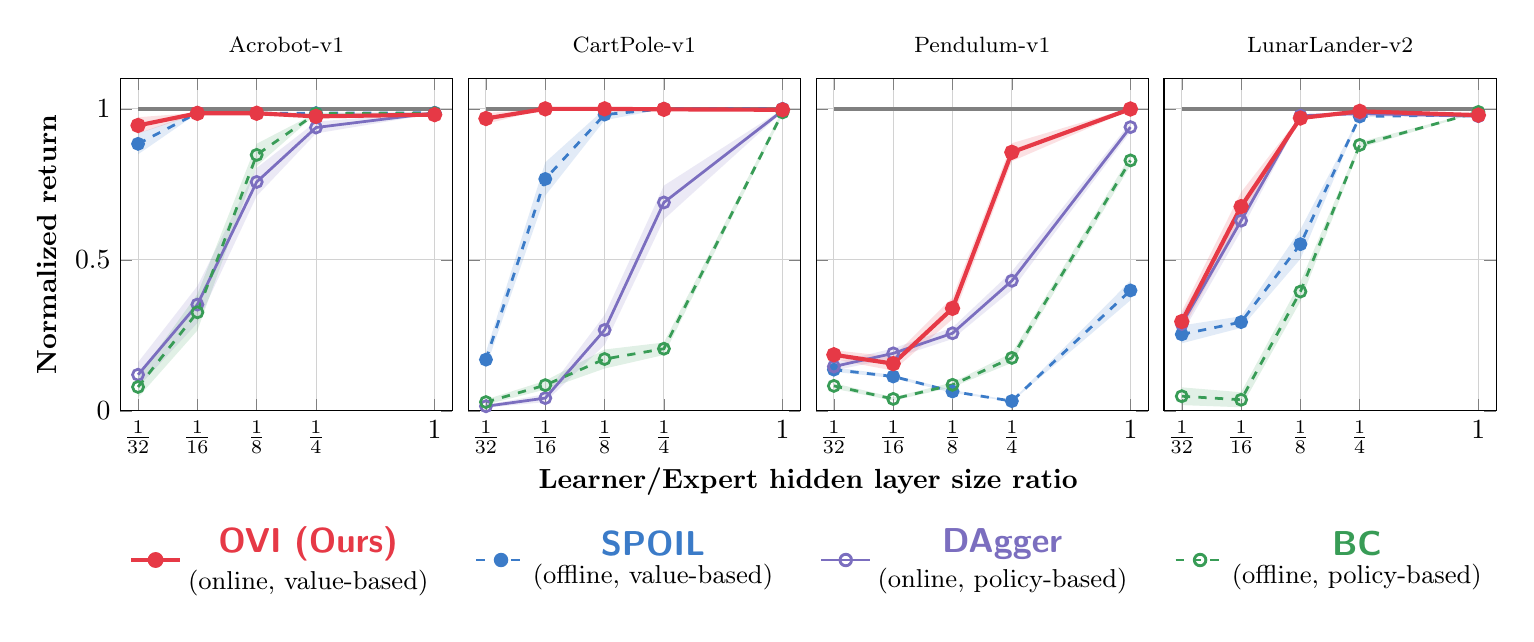
\begin{tikzpicture}
  \begin{groupplot}[
    size plot,
    group style={
      group size=4 by 1,
      horizontal sep=0.2cm,
      xlabels at=edge bottom,
      ylabels at=edge left,
    },
  ]
  \nextgroupplot[
    title={Acrobot-v1},
    ymin=0,
    ymax=1.1,
    ylabel={Normalized return},
    legend to name=sharedlegend,
    legend columns=4,
    legend style={draw=none,font=\small,/tikz/every even column/.append style={column sep=0.5cm}}
  ]
    \addlegendimage{algcol3, solid, mark=*, mark size=2.0pt, line width=1.5pt}
    \addlegendentry{\shortstack[c]{{\large\textcolor{algcol3}{\textbf{\textsf{OVI (Ours)}}}}\\(online, value-based)}}
    \addplot[gray, solid, line width=1.5pt, forget plot] coordinates {(2, 1) (64, 1)};
    \addplot[name path=pu0, draw=none, forget plot] coordinates { (2,0.9187) (4,0.9878) (8,0.9870) (16,0.9876) (64,0.9885) };
    \addplot[name path=pl0, draw=none, forget plot] coordinates { (2,0.8494) (4,0.9851) (8,0.9836) (16,0.9840) (64,0.9854) };
    \addplot[fill=algcol0, fill opacity=0.15, draw=none, forget plot] fill between[of=pu0 and pl0];
    \addplot[algcol0, dashed, mark=*, mark size=2.0pt, line width=1.0pt, opacity=1.0, mark options={solid}] coordinates { (2,0.8841) (4,0.9864) (8,0.9853) (16,0.9858) (64,0.9869) };
    \addlegendentry{\shortstack[c]{{\large\textcolor{algcol0}{\textbf{\textsf{SPOIL}}}}\\(offline, value-based)}}
    \addplot[name path=pu1, draw=none, forget plot] coordinates { (2,0.1605) (4,0.4130) (8,0.8046) (16,0.9577) (64,0.9892) };
    \addplot[name path=pl1, draw=none, forget plot] coordinates { (2,0.0784) (4,0.2908) (8,0.7113) (16,0.9185) (64,0.9843) };
    \addplot[fill=algcol1, fill opacity=0.15, draw=none, forget plot] fill between[of=pu1 and pl1];
    \addplot[algcol1, solid, mark=o, mark size=2.0pt, line width=1.0pt, opacity=1.0, mark options={fill=white, solid}] coordinates { (2,0.1195) (4,0.3519) (8,0.7579) (16,0.9381) (64,0.9867) };
    \addlegendentry{\shortstack[c]{{\large\textcolor{algcol1}{\textbf{\textsf{DAgger}}}}\\(online, policy-based)}}
    \addplot[name path=pu2, draw=none, forget plot] coordinates { (2,0.1139) (4,0.3864) (8,0.8845) (16,0.9863) (64,0.9875) };
    \addplot[name path=pl2, draw=none, forget plot] coordinates { (2,0.0441) (4,0.2660) (8,0.8105) (16,0.9825) (64,0.9837) };
    \addplot[fill=algcol2, fill opacity=0.15, draw=none, forget plot] fill between[of=pu2 and pl2];
    \addplot[algcol2, dashed, mark=o, mark size=2.0pt, line width=1.0pt, opacity=1.0, mark options={fill=white, solid}] coordinates { (2,0.0790) (4,0.3262) (8,0.8475) (16,0.9844) (64,0.9856) };
    \addlegendentry{\shortstack[c]{{\large\textcolor{algcol2}{\textbf{\textsf{BC}}}}\\(offline, policy-based)}}
    \addplot[name path=pu3, draw=none, forget plot] coordinates { (2,0.9723) (4,0.9869) (8,0.9886) (16,0.9783) (64,0.9835) };
    \addplot[name path=pl3, draw=none, forget plot] coordinates { (2,0.9176) (4,0.9834) (8,0.9822) (16,0.9718) (64,0.9781) };
    \addplot[fill=algcol3, fill opacity=0.15, draw=none, forget plot] fill between[of=pu3 and pl3];
    \addplot[algcol3, solid, mark=*, mark size=2.0pt, line width=1.5pt, opacity=1.0, mark options={solid}, forget plot] coordinates { (2,0.9450) (4,0.9852) (8,0.9854) (16,0.9751) (64,0.9808) };
  \nextgroupplot[
    title={CartPole-v1},
    ymin=0,
    ymax=1.1,
    yticklabels={}
  ]
    \addplot[gray, solid, line width=1.5pt, forget plot] coordinates {(2, 1) (64, 1)};
    \addplot[name path=pu4, draw=none, forget plot] coordinates { (2,0.1948) (4,0.8228) (8,0.9998) (16,1.0000) (64,1.0000) };
    \addplot[name path=pl4, draw=none, forget plot] coordinates { (2,0.1442) (4,0.7128) (8,0.9623) (16,1.0000) (64,1.0000) };
    \addplot[fill=algcol0, fill opacity=0.15, draw=none, forget plot] fill between[of=pu4 and pl4];
    \addplot[algcol0, dashed, mark=*, mark size=2.0pt, line width=1.0pt, opacity=1.0, mark options={solid}] coordinates { (2,0.1695) (4,0.7678) (8,0.9810) (16,1.0000) (64,1.0000) };
    \addplot[name path=pu5, draw=none, forget plot] coordinates { (2,0.0197) (4,0.0552) (8,0.3174) (16,0.7459) (64,0.9984) };
    \addplot[name path=pl5, draw=none, forget plot] coordinates { (2,0.0104) (4,0.0289) (8,0.2183) (16,0.6341) (64,0.9897) };
    \addplot[fill=algcol1, fill opacity=0.15, draw=none, forget plot] fill between[of=pu5 and pl5];
    \addplot[algcol1, solid, mark=o, mark size=2.0pt, line width=1.0pt, opacity=1.0, mark options={fill=white, solid}] coordinates { (2,0.0151) (4,0.0421) (8,0.2678) (16,0.6900) (64,0.9940) };
    \addplot[name path=pu6, draw=none, forget plot] coordinates { (2,0.0375) (4,0.0995) (8,0.2030) (16,0.2262) (64,0.9971) };
    \addplot[name path=pl6, draw=none, forget plot] coordinates { (2,0.0203) (4,0.0705) (8,0.1400) (16,0.1849) (64,0.9794) };
    \addplot[fill=algcol2, fill opacity=0.15, draw=none, forget plot] fill between[of=pu6 and pl6];
    \addplot[algcol2, dashed, mark=o, mark size=2.0pt, line width=1.0pt, opacity=1.0, mark options={fill=white, solid}] coordinates { (2,0.0289) (4,0.0850) (8,0.1715) (16,0.2056) (64,0.9882) };
    \addplot[name path=pu7, draw=none, forget plot] coordinates { (2,0.9861) (4,1.0000) (8,1.0000) (16,0.9999) (64,0.9999) };
    \addplot[name path=pl7, draw=none, forget plot] coordinates { (2,0.9499) (4,1.0000) (8,1.0000) (16,0.9968) (64,0.9939) };
    \addplot[fill=algcol3, fill opacity=0.15, draw=none, forget plot] fill between[of=pu7 and pl7];
    \addplot[algcol3, solid, mark=*, mark size=2.0pt, line width=1.5pt, opacity=1.0, mark options={solid}, forget plot] coordinates { (2,0.9680) (4,1.0000) (8,1.0000) (16,0.9984) (64,0.9969) };
  \nextgroupplot[
    title={Pendulum-v1},
    ymin=0,
    ymax=1.1,
    yticklabels={}
  ]
    \addplot[gray, solid, line width=1.5pt, forget plot] coordinates {(2, 1) (64, 1)};
    \addplot[name path=pu8, draw=none, forget plot] coordinates { (2,0.1437) (4,0.1188) (8,0.0688) (16,0.0340) (64,0.4311) };
    \addplot[name path=pl8, draw=none, forget plot] coordinates { (2,0.1291) (4,0.1086) (8,0.0592) (16,0.0304) (64,0.3660) };
    \addplot[fill=algcol0, fill opacity=0.15, draw=none, forget plot] fill between[of=pu8 and pl8];
    \addplot[algcol0, dashed, mark=*, mark size=2.0pt, line width=1.0pt, opacity=1.0, mark options={solid}] coordinates { (2,0.1364) (4,0.1137) (8,0.0640) (16,0.0322) (64,0.3986) };
    \addplot[name path=pu9, draw=none, forget plot] coordinates { (2,0.1596) (4,0.2068) (8,0.2758) (16,0.4614) (64,0.9550) };
    \addplot[name path=pl9, draw=none, forget plot] coordinates { (2,0.1335) (4,0.1738) (8,0.2379) (16,0.3999) (64,0.9239) };
    \addplot[fill=algcol1, fill opacity=0.15, draw=none, forget plot] fill between[of=pu9 and pl9];
    \addplot[algcol1, solid, mark=o, mark size=2.0pt, line width=1.0pt, opacity=1.0, mark options={fill=white, solid}] coordinates { (2,0.1466) (4,0.1903) (8,0.2569) (16,0.4306) (64,0.9395) };
    \addplot[name path=pu10, draw=none, forget plot] coordinates { (2,0.0914) (4,0.0451) (8,0.0939) (16,0.1916) (64,0.8464) };
    \addplot[name path=pl10, draw=none, forget plot] coordinates { (2,0.0735) (4,0.0336) (8,0.0783) (16,0.1588) (64,0.8119) };
    \addplot[fill=algcol2, fill opacity=0.15, draw=none, forget plot] fill between[of=pu10 and pl10];
    \addplot[algcol2, dashed, mark=o, mark size=2.0pt, line width=1.0pt, opacity=1.0, mark options={fill=white, solid}] coordinates { (2,0.0825) (4,0.0393) (8,0.0861) (16,0.1752) (64,0.8292) };
    \addplot[name path=pu11, draw=none, forget plot] coordinates { (2,0.2008) (4,0.1793) (8,0.3753) (16,0.8861) (64,1.0030) };
    \addplot[name path=pl11, draw=none, forget plot] coordinates { (2,0.1704) (4,0.1331) (8,0.3033) (16,0.8263) (64,0.9961) };
    \addplot[fill=algcol3, fill opacity=0.15, draw=none, forget plot] fill between[of=pu11 and pl11];
    \addplot[algcol3, solid, mark=*, mark size=2.0pt, line width=1.5pt, opacity=1.0, mark options={solid}, forget plot] coordinates { (2,0.1856) (4,0.1562) (8,0.3393) (16,0.8562) (64,0.9995) };
  \nextgroupplot[
    title={LunarLander-v2},
    ymin=0,
    ymax=1.1,
    yticklabels={}
  ]
    \addplot[gray, solid, line width=1.5pt, forget plot] coordinates {(2, 1) (64, 1)};
    \addplot[name path=pu12, draw=none, forget plot] coordinates { (2,0.2827) (4,0.3131) (8,0.6009) (16,0.9769) (64,0.9820) };
    \addplot[name path=pl12, draw=none, forget plot] coordinates { (2,0.2236) (4,0.2745) (8,0.5029) (16,0.9724) (64,0.9792) };
    \addplot[fill=algcol0, fill opacity=0.15, draw=none, forget plot] fill between[of=pu12 and pl12];
    \addplot[algcol0, dashed, mark=*, mark size=2.0pt, line width=1.0pt, opacity=1.0, mark options={solid}] coordinates { (2,0.2532) (4,0.2938) (8,0.5519) (16,0.9747) (64,0.9806) };
    \addplot[name path=pu13, draw=none, forget plot] coordinates { (2,0.3207) (4,0.6632) (8,0.9818) (16,0.9886) (64,0.9808) };
    \addplot[name path=pl13, draw=none, forget plot] coordinates { (2,0.2541) (4,0.5961) (8,0.9730) (16,0.9795) (64,0.9705) };
    \addplot[fill=algcol1, fill opacity=0.15, draw=none, forget plot] fill between[of=pu13 and pl13];
    \addplot[algcol1, solid, mark=o, mark size=2.0pt, line width=1.0pt, opacity=1.0, mark options={fill=white, solid}] coordinates { (2,0.2874) (4,0.6297) (8,0.9774) (16,0.9841) (64,0.9756) };
    \addplot[name path=pu14, draw=none, forget plot] coordinates { (2,0.0777) (4,0.0615) (8,0.4274) (16,0.8904) (64,0.9909) };
    \addplot[name path=pl14, draw=none, forget plot] coordinates { (2,0.0189) (4,0.0118) (8,0.3623) (16,0.8706) (64,0.9886) };
    \addplot[fill=algcol2, fill opacity=0.15, draw=none, forget plot] fill between[of=pu14 and pl14];
    \addplot[algcol2, dashed, mark=o, mark size=2.0pt, line width=1.0pt, opacity=1.0, mark options={fill=white, solid}] coordinates { (2,0.0483) (4,0.0366) (8,0.3949) (16,0.8805) (64,0.9898) };
    \addplot[name path=pu15, draw=none, forget plot] coordinates { (2,0.3294) (4,0.7242) (8,0.9770) (16,0.9943) (64,0.9837) };
    \addplot[name path=pl15, draw=none, forget plot] coordinates { (2,0.2621) (4,0.6284) (8,0.9622) (16,0.9893) (64,0.9748) };
    \addplot[fill=algcol3, fill opacity=0.15, draw=none, forget plot] fill between[of=pu15 and pl15];
    \addplot[algcol3, solid, mark=*, mark size=2.0pt, line width=1.5pt, opacity=1.0, mark options={solid}, forget plot] coordinates { (2,0.2957) (4,0.6763) (8,0.9696) (16,0.9918) (64,0.9792) };
  \end{groupplot}
  % Centered single X-label
  \node[below=0.6cm, font=\normalsize\bfseries] at ($(group c2r1.south east)!0.5!(group c3r1.south west)$) {Learner/Expert hidden layer size ratio};
  % Single legend spanning the full combined plot width
  \newlength{\groupplotwidth}
  \pgfextractx{\groupplotwidth}{\pgfpointdiff{\pgfpointanchor{group c1r1}{west}}{\pgfpointanchor{group c4r1}{east}}}
  \node[below=1.2cm, anchor=north] at ($(group c1r1.south west)!0.5!(group c4r1.south east)$) {%
    \resizebox{\groupplotwidth}{!}{\pgfplotslegendfromname{sharedlegend}}%
  };
  \end{tikzpicture}
\end{document}